\documentclass[10pt,conference]{IEEEtran}
\IEEEoverridecommandlockouts

\usepackage{cite}
\usepackage{amsmath,amssymb,amsfonts}
\usepackage{algorithmic}
\usepackage{graphicx}
% \usepackage{subcaption}
% \usepackage{subfig}
\usepackage{textcomp}
\usepackage{xcolor}
\usepackage{subfig}
\usepackage{listings}

% \usepackage{subcaption}
\lstset{numbers=left,stepnumber=1,basicstyle=\footnotesize\ttfamily}
\def\BibTeX{{\rm B\kern-.05em{\sc i\kern-.025em b}\kern-.08em
T\kern-.1667em\lower.7ex\hbox{E}\kern-.125emX}}
\def\code#1{\texttt{#1}}

\makeatletter
\def\endthebibliography{%
  \def\@noitemerr{\@latex@warning{Empty `thebibliography' environment}}%
  \endlist
}
\makeatother

\begin{document}

\title{Comparing Machine Learning Algorithms for Predicting Cancellation of Hotel Bookings\\}

\author{\IEEEauthorblockN{Kevin de Haan}
  \IEEEauthorblockA{ %\textit{Department of Computing Science} \\
%     \textit{University of Alberta}\\
    Edmonton, Canada\\
  Email: kdehaan@ualberta.ca}
}

\maketitle

\begin{abstract}
 Hotels around the world have dealt with cancellations since their inception. Reservations require that a space be set aside, and cancellations mean that even the most consistently popular vacation destinations are often floating unused rooms and wasted space. Being able to predict whether a customer is likely to cancel ahead of time allows establishments to operate on significantly tighter occupancy margins, improving their efficiency and freeing up more space for customers who will follow through on their plans. The nature of this binary classification problem is well suited to many simple machine learning strategies.
\end{abstract}

\begin{IEEEkeywords}
  Data Science; Hospitality Industry; Machine Learning; K-nearest Neighbors; Linear SGD; Multi-layer Perceptron; Scikit-learn
\end{IEEEkeywords}


\section{Introduction}
  In the hospitality industry, it is paramount to maximize occupancy rates. Cancellations can have a significant impact on revenue, and to compensate many hotels often sell above their capacity\cite{mehrotra_ruttley_2006}. While this practice is often worthwhile, it can have significant costs in relocation, compensation and reputation. Having the ability to predict the likelihood of cancellation on a case-by-case basis has significant impact on reducing the risk and improving the margins involved with overbooking a hotel or resort\cite{morales2010}. One might expect that the factors leading to cancelling a hotel reservation would extremely complicated, akin to predicting the weather; however, the majority of cancelled bookings are in fact predictable given a relatively small subset of information. Using the hotel booking data set created by Antonio, de Almeida and Nunes\cite{Antonio2019} we will investigate the utility of three off-the-shelf machine learning algorithms for predicting the outcome of a hotel reservation.

\section{Problem Formulation}
  Simply put, the goal of each of the machine learning models used is to take in a set of parameters that can be known before the date of arrival, and make a binary prediction about whether the reservation is going to be cancelled.
  \subsection{The Data}
    The data set used is adapted from one created by Antonio, de Almeida and Nunes\cite{Antonio2019} that has been cleaned and formatted by Mock and Bichat\cite{mock_bichat}. It includes bookings from two locations - a city hotel and a resort hotel. Data columns include the lead time between booking and the date of stay, the date of arrival, the duration of the stay, the volume of adults, children and babies, if the guest is a repeat customer, the number of previous cancellations and amount of special requests made, among others. 66\% of the rows are taken from the city hotel, while the remaining 34\% are from the resort hotel. There are 44224 (37.06\%) examples of cancelled bookings and 75116 (62.94\%) instances where the booking went through, for a total of 11934 rows. Some columns have been altered to preserve anonymity\cite{Antonio2019}.
  
  

\section{Approaches and Baselines}
  For the purposes of this experiment, three machine learning approaches will be evaluated:
  \begin{itemize}
    \item \textbf{\emph{k}-nearest Neighbors} (KNN) classification uses the training data to establish a vector space that an input instance can be compared to in order to obtain a class prediction. Essentially, \emph{k}-nearest neighbors acts similarly to an Voronoi diagram where each input point is classified by the closest existing point. In fact, if the hyperparameter \emph{n\_neighbors} is set to 1 the classifier works exactly as an \emph{n}-dimensional Voronoi cell. With the hyperparameters selected during parameter tuning, the \emph{k}-nearest Neighbors classifier used in this experiment considers the nearest 20 neighbors weighted by their Manhattan distance. In order to improve the efficiency of spacial searches, the points are separated into a \emph{k}-dimensional tree with 30 items per leaf. One of the biggest weaknesses of this model is that it requires full computation of the nearest neighbor upon each usage as a classifier - there is no way to produce a 'final' version of the model, as it is purely a statistical evaluation tool.
    \item A \textbf{Linear Classifier} trained using \textbf{Stochastic Gradient Descent} (SGD). With the selected hyperparameters, the classifier is a linear SVM using a quadratically penalized (\emph{squared\_hinge}) loss function and \emph{l2} regularization. As a binary classification problem, an SVM has the potential to be one of the best out-of-the-box tools available; however, the results will depend on if the problem is intrinsically linearly separable. The SGD component of the classifier is used to iteratively minimize an objective function by calculating and following a gradient and 'descending' towards the local (or ideally global) minimum. As a result of the minimized objective function, the model can produce an optimized hyperplane used to separate the input vector space for predicting class outputs. The most significant weakness of this technique is that if there are many different 'sets' of circumstances (almost like subclasses) which can cause bookings to be cancelled it may have trouble finding an appropriate hyperplane.
    \item A \textbf{Multi-layer Perceptron} (MLP) is a feedforward neural network consisting of (at least) an input layer, a hidden layer, and an output layer of nodes (or \emph{perceptrons}). As a nonlinear classifier (and unlike the linear SVM), the MLP model is capable of correctly predicting the classes of data that is not linearly separable. With the selected hyperparameters, this MLP uses a \emph{rectified linear unit} (RELU) activation function and the \emph{adaptive moment estimation} (\emph{Adam}) optimization algorithm. \emph{Adam} is an improved version of stochastic gradient descent which maintains a learning rate for each network parameter instead of all weight updates as a whole\cite{Kingma2015AdamAM}. Additionally, it considers estimates of the first and second moments of the learning rate gradients\cite{Kingma2015AdamAM}.
  \end{itemize}
  For each of these approaches, hyperparameter selection was performed using a search through a parameter grid.

  In addition to the machine learning techniques employed, a baseline must be established. As this is a \emph{k}-category classification problem, each approach will be compared to two naive baseline predictors:
  \begin{itemize}
    \item \textbf{Majority Guess} will always predict that a booking will not be cancelled.
    \item \textbf{Uniform Random Guess} will predict each possible classification category (i.e, cancelled and not cancelled) at an equal rate.
  \end{itemize}
  

\section{Evaluating Performance}
 While the relatively low class imbalance of this binary classification problem means that raw accuracy is still meaningful, it is still preferable to find a different metric to better represent the trade-off between precision and recall. Towards this end, the models are evaluated primarily using the \emph{Area Under the Receiver Operating Characteristic Curve} (ROC AUC), a tool used specifically for determining the predictive ability of a binary classifier as the threshold between precision and recall is varied\cite{Fawcett2006}. For this metric, a perfect score is 1 while the worst possible score is 0.5 (this is because in a binary classifier, being 0\% correct is equivalent to being 100\% correct). In addition to the ROC AUC, the \emph{f\textsubscript{1}} score\cite{rijsbergen_1995} and raw accuracy are also included in the event that the reader is more comfortable with their relative values.
 
 Note that both of the naive predictors (\emph{majority guess} and \emph{uniform random guess}) will produce an ROC AUC score of very nearly 0.5, and very poor \emph{f\textsubscript{1}} scores (0 and 0.425 respectively).

\section{Results}

\begin{figure}
  \centering
  \subfloat[KNN\label{knn_learn}]{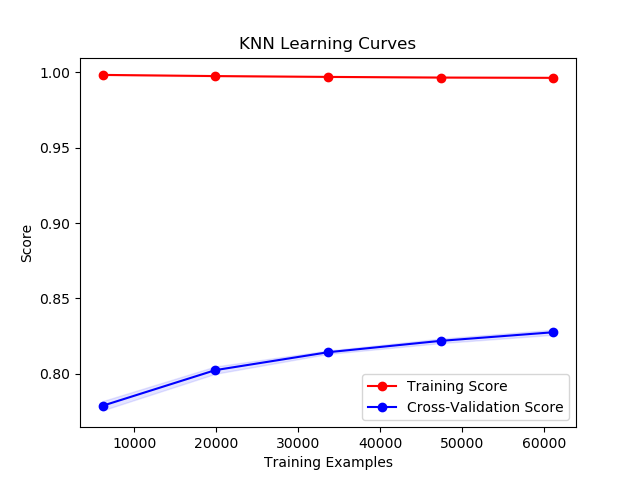
\includegraphics[width=0.25\textwidth]{figures/KNN_learning_curve.png}} \\
  \subfloat[SGD SVM\label{sgd_learn}]{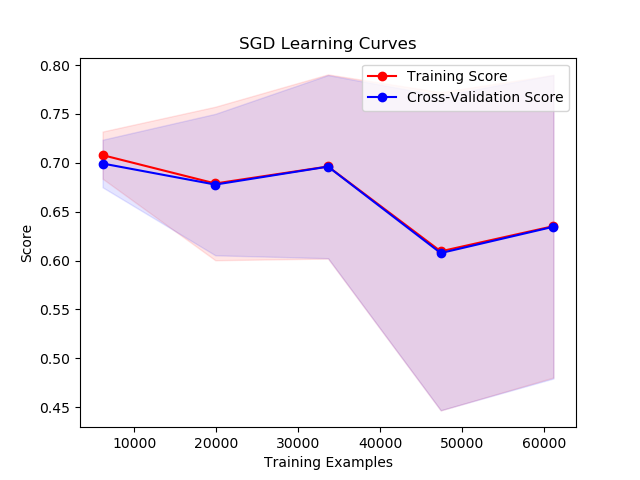
\includegraphics[width=0.25\textwidth]{figures/SGD_learning_curve.png}}
  \subfloat[MLP\label{mlp_learn}]{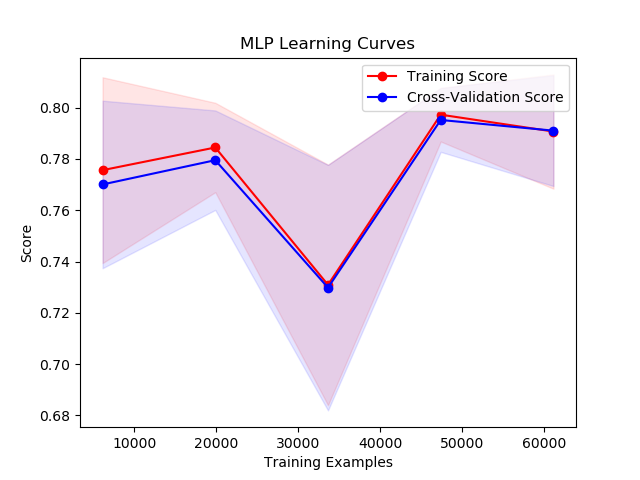
\includegraphics[width=0.25\textwidth]{figures/MLP_learning_curve.png}}
  \caption{Learning Curves}
  \label{learning_curves}
\end{figure}

In training, the KNN predictor benefited most from increasingly large amounts of training examples as seen in figure \ref{knn_learn}. The SVM demonstrated little improvement with additional training examples, possibly due to the data set being fundamentally non-linear. Finally, while the MLP at first glance appears to have been wildly fluctuating, note that the bounds of figure \ref{mlp_learn} are over a smaller interval than that of the linear classifier.

\begin{figure}
  \centering
  \subfloat[KNN\label{knn_roc}]{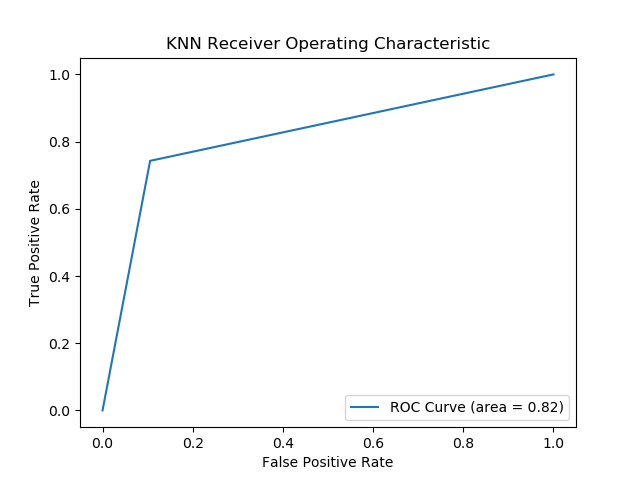
\includegraphics[width=0.25\textwidth]{figures/KNN_roc_auc.png}} \\
  \subfloat[SGD SVM\label{sgd_roc}]{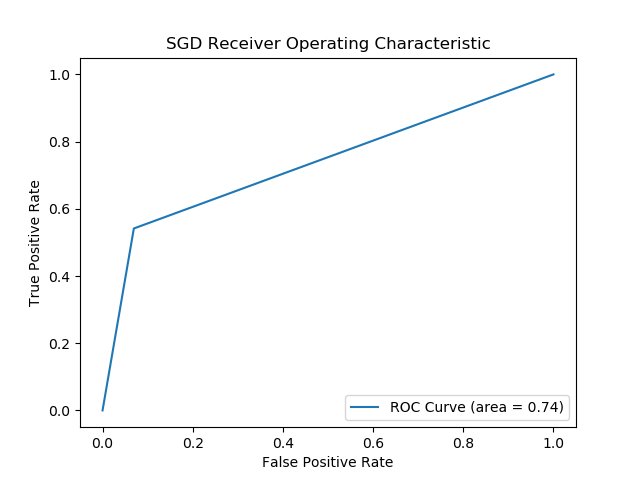
\includegraphics[width=0.25\textwidth]{figures/SGD_roc_auc.png}}
  \subfloat[MLP\label{mlp_roc}]{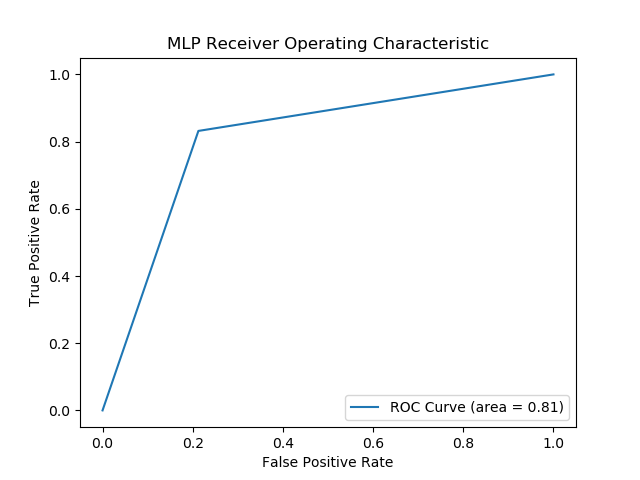
\includegraphics[width=0.25\textwidth]{figures/MLP_roc_auc.png}}
  \caption{Receiver Operating Characteristic (ROC) Curves}
  \label{roc_plot}
\end{figure}

Figures \ref{knn_roc} and \ref{mlp_roc} display highly similar tradeoff curves between true positives and false positives, as well as highly similar values for the area under the receiver operating characteristic curve (ROC AUC), the primary performance metric used during training. Of note, in the intermediate point of each curve the KNN has a tendency towards a lower false positive rate while the MLP displays a better true positive rate. The linear classifier in figure \ref{sgd_roc} does a reasonable job at avoiding false positives yet fails to classify true positives as well as the other models, performing noticeably worse overall.


\begin{table}
  \centering
  \begin{tabular}{c|c c c}
    & ROC AUC & \emph{f\textsubscript{1}} Score & Accuracy \\
    \hline
    \hline
    KNN & 0.818 & 0.772 & 0.838 \\
    SGD & 0.732 & 0.645 & 0.785 \\
    MLP & 0.810 & 0.758 & 0.804 \\
    \hline
    Majority & 0.500 & 0.000 & 0.631 \\
    Uniform & 0.499 & 0.424 & 0.499 \\

  \end{tabular}
  \caption{Test performance of the three sampled classifiers. For each performance metric, values closer to 1 are preferable.}
  \label{resultsummary}
\end{table}

\section{Conclusion}
  While all three of the models performed significantly better than both of the baseline estimators, it is curious to observe that the \emph{k}-nearest Neighbors algorithm outperformed both of the other two classification engines, even if only slightly in the case of the MLP classifier. In the case of the SGD-trained linear classifier this is best explained by the problem set simply not being linearly separable and therefore impossible to obtain a perfect model of the situation. However, the MLP should generally be able to outperform the KNN model in most cases, and it is likely that the greatest limiting factor in this instance was my own skill and experience with hyperparameter tuning. The SGD-trained linear classifier would also almost certainly benefit from a more experienced touch, while the KNN system is likely simple enough to have little tuning required.

  Even considering the slightly reduced effectiveness of the amateur MLP compared to the KNN classifier, it would likely be preferable to use the MLP in any sort of real applications due to the fact that it is significantly less computationally expensive to use as a classifier once trained, as well as being more flexible to the introduction of additional data columns. 

  Ultimately, while the exhibited performance likely has significant room for improvement, a classifier such as the KNN or MLP models trained in this experiment would still be a very powerful tool for any hotel attempting to practice efficient overbooking - being able to predict individual bookings at 80\% accuracy is a drastic improvement compared to simply assuming 34\% of bookings will be cancelled.

\nocite{*}
\bibliography{bibs/refs}
\bibliographystyle{IEEEtran}


\vspace{12pt}

\end{document}